\section{Certificates}\label{app:certificates}

\subsection{Strong deletion sequences}
The following sequences, produced by \texttt{tools/strong\_contractible.py --trace} (an exact search independent of the C program), reduce $\Ga+\{0,1\}$, $\Gb+\{0,3\}$, $\Gc+\{2,3\}$ and $\Dunce+\{9,12\}$ to $K_1$. Each line deletes a vertex $v$ with $\Nb(v)\in\IS$ or an edge $uv$ with $\Nb(u,v)\in\IS$ in the current graph; the reader may check each step with any of the tools in the repository.

{\scriptsize\verbatiminput{appendix_data/traces.txt}}

Figures~\ref{fig:certb} and~\ref{fig:certc} show the sequences for $\Gb+\{0,3\}$ and $\Gc+\{2,3\}$ step by step, as Fig.~\ref{fig:cert} does for $\Ga+\{0,1\}$.

\begin{figure}[p]\centering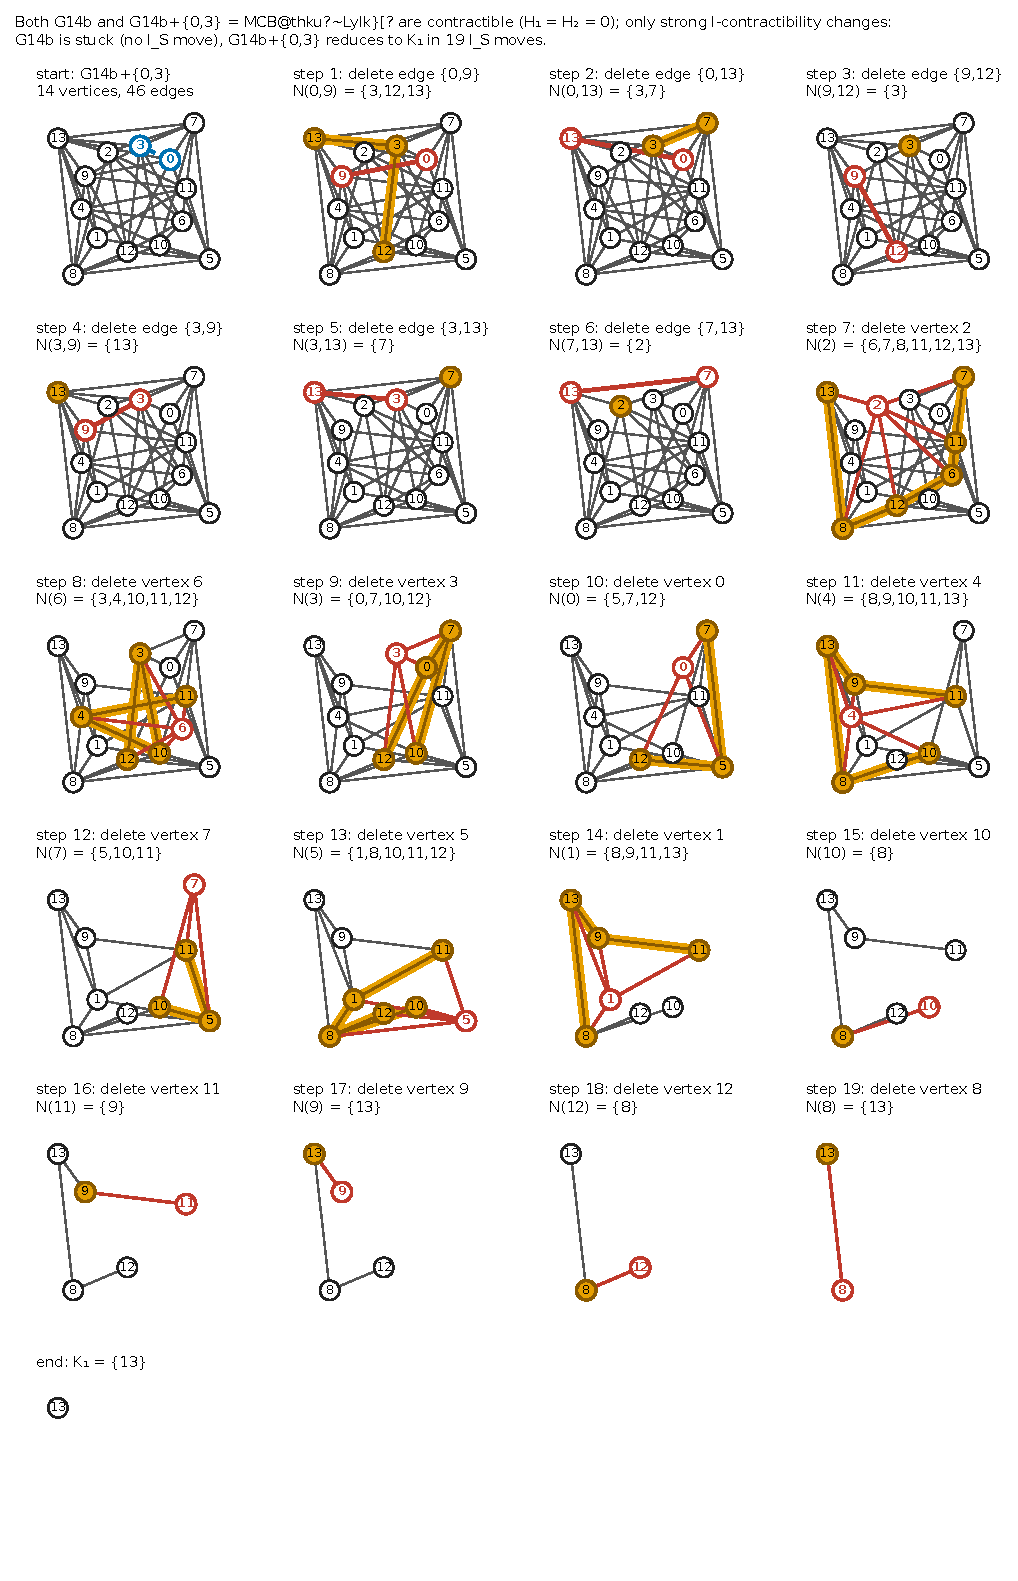
\includegraphics[height=0.90\textheight]{figures/fig06b.pdf}\caption{Certificate that $\Gb+\{0,3\}\in\IS$ ($19$ strong deletions).}\label{fig:certb}\end{figure}
\begin{figure}[p]\centering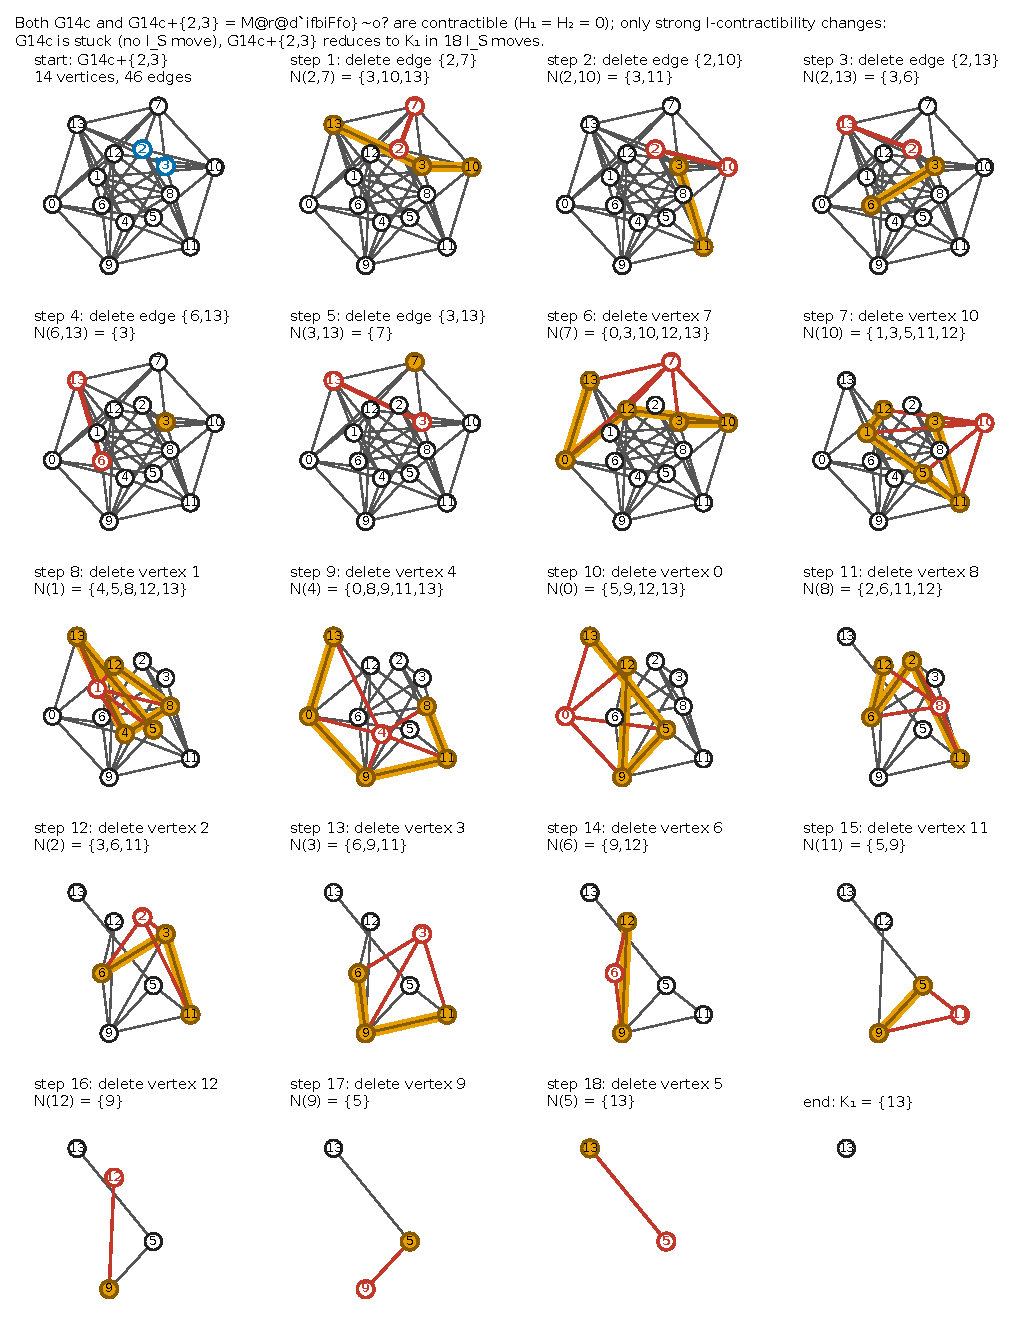
\includegraphics[height=0.90\textheight]{figures/fig06c.pdf}\caption{Certificate that $\Gc+\{2,3\}\in\IS$ ($18$ strong deletions).}\label{fig:certc}\end{figure}

\subsection{Routes to a cone (Proposition~\ref{prop:frias})}
Adding the following edges in order, each with common neighbourhood in $\IS$ at the moment of addition, turns the graph into a cone with the indicated apex (verified by \texttt{tools/strong\_contractible.py}):
\begin{itemize}[leftmargin=2em]
\item $\Ga$: $\{0,1\}$, $\{8,13\}$, $\{0,7\}$, $\{1,4\}$, $\{4,7\}$, $\{7,9\}$, $\{6,9\}$, $\{6,13\}$, $\{11,13\}$, $\{5,13\}$, $\{12,13\}$; apex $13$.
\item $\Gb$: $\{0,3\}$, $\{3,5\}$, $\{10,12\}$, $\{0,10\}$, $\{0,6\}$, $\{6,8\}$, $\{1,10\}$, $\{1,4\}$, $\{10,11\}$, $\{2,10\}$, $\{10,13\}$, $\{9,10\}$; apex $10$.
\item $\Gc$: $\{0,11\}$, $\{2,3\}$, $\{2,9\}$, $\{6,11\}$, $\{8,9\}$, $\{0,8\}$, $\{3,8\}$, $\{0,1\}$, $\{0,10\}$, $\{0,2\}$, $\{0,3\}$, $\{0,6\}$; apex $0$.
\item $\Dunce$: $\{2,4\}$, $\{3,5\}$, $\{2,8\}$, $\{9,12\}$, $\{5,7\}$, $\{1,7\}$, $\{7,10\}$, $\{0,7\}$; apex $7$.
\end{itemize}

\subsection{Integer homology}
\texttt{certificates/integer\_homology.txt} lists, for the three graphs of Theorem~\ref{thm:A}, the $51$ stuck graphs and $\Dunce$, the number of simplices in each dimension, the $\Ztwo$-Betti numbers and the integer homology groups computed by Smith normal form with \texttt{tools/clique\_homology.py}.

\FloatBarrier
